\documentclass[a4paper,10pt]{article}

\usepackage[top=0.75in, bottom=0.2in, left=0.35in, right=0.35in]{geometry}
\usepackage{graphicx}  % 用于插入图片
\usepackage{booktabs}
\usepackage{url}
\usepackage{enumitem}
\usepackage{palatino}
\usepackage{tabularx}
\usepackage[UTF8]{ctex}  % 支持中文
\usepackage{xcolor} % 用于定义和使用颜色
\fontfamily{SansSerif}
\selectfont

\usepackage[T1]{fontenc}
\usepackage
%[ansinew]
[utf8]
{inputenc}

\definecolor{mygrey}{gray}{0.82}
\textheight=9.75in
\raggedbottom

\setlength{\tabcolsep}{0in}
\newcommand{\isep}{-2 pt}
\newcommand{\lsep}{-0.5cm}
\newcommand{\psep}{-0.6cm}
\renewcommand{\labelitemii}{$\circ$}

\pagestyle{empty}
%-----------------------------------------------------------
%Custom commands
\newcommand{\resitem}[1]{\item #1 \vspace{-2pt}}
\newcommand{\resheading}[1]{{\small \colorbox{mygrey}{\begin{minipage}{0.99\textwidth}{\textbf{#1 \vphantom{p\^{E}}}}\end{minipage}}}}
\newcommand{\ressubheading}[3]{
\begin{tabular*}{6.62in}{l @{\extracolsep{\fill}} r}
	\textsc{{\textbf{#1}}} & \textsc{\textit{[#2]}} \\
\end{tabular*}\vspace{-8pt}}
%-----------------------------------------------------------

% 定义 4 种逐渐变浅的浅蓝色
\definecolor{LightBlue1}{RGB}{173, 216, 230} % 浅蓝色 1
\definecolor{LightBlue2}{RGB}{191, 223, 235} % 浅蓝色 2
\definecolor{LightBlue3}{RGB}{209, 230, 240} % 浅蓝色 3
\definecolor{LightBlue4}{RGB}{227, 237, 245} % 浅蓝色 4

\begin{document}

% 第一份：最深的浅蓝色
% Header with Photo
\begin{table}
    \begin{minipage}{0.15\linewidth}
        % 插入照片
        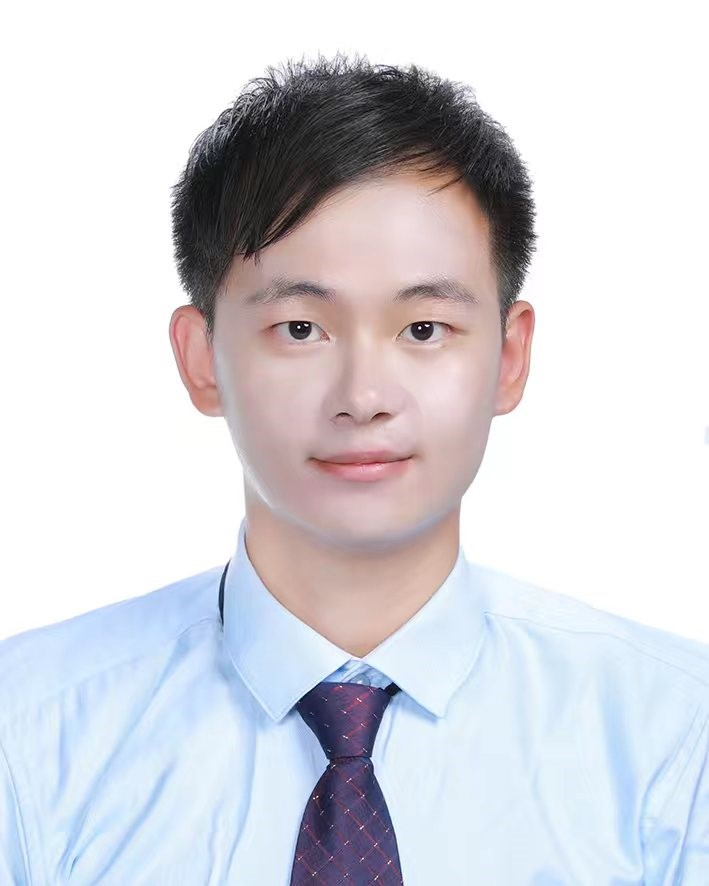
\includegraphics[width=\linewidth]{pic.png}  % 照片路径
    \end{minipage}
    \begin{minipage}{0.65\linewidth}
        \setlength{\tabcolsep}{70pt}
        \def\arraystretch{1.15}
        \begin{tabular}{ll}
            \textbf{\Large{张文杰}}  &  {17704240848} \\
            \textbf{香港科技大学} & \textbf{生命科学 \& 化学} \\
            中共党员 &  \\
        \end{tabular}
    \end{minipage}\hfill
\end{table}

% 联系方式背景颜色替换
\noindent \colorbox{LightBlue1}{\begin{minipage}{0.99\textwidth}{\textbf{联系方式 \vphantom{p\^{E}}}}\end{minipage}}\\[-0.3cm]
\begin{itemize}[noitemsep,nolistsep]
    \item 邮箱: 17704240848@163.com
    \item 微信: 17704240848
    \item 电话: 17704240848
    \item GitHub: jayzyzy
\end{itemize}

% 第二份：稍浅的浅蓝色
\newpage
\begin{table}
    \begin{minipage}{0.15\linewidth}
        % 插入照片
        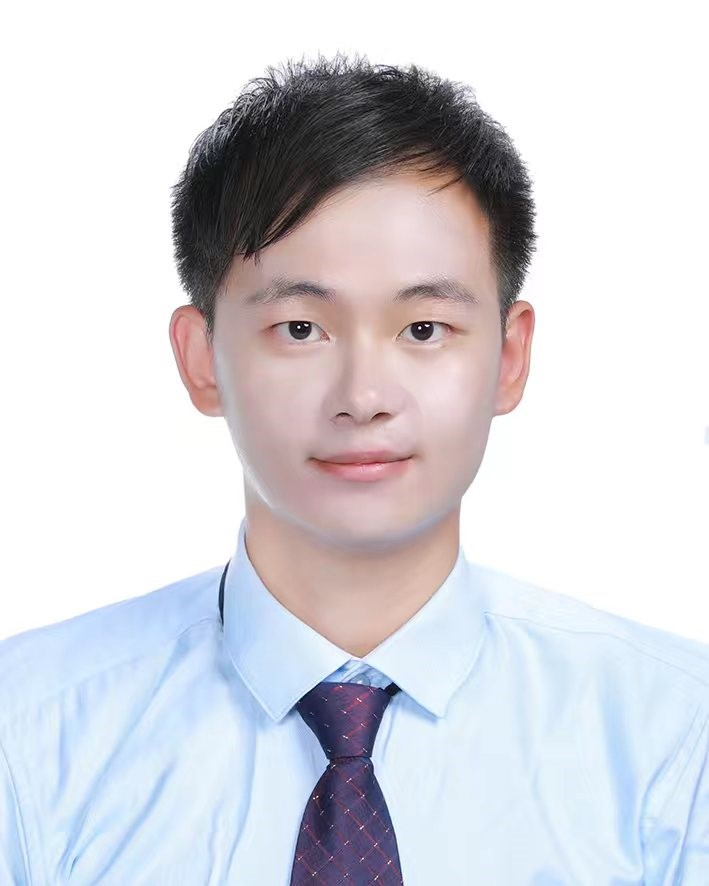
\includegraphics[width=\linewidth]{pic.png}  % 照片路径
    \end{minipage}
    \begin{minipage}{0.65\linewidth}
        \setlength{\tabcolsep}{70pt}
        \def\arraystretch{1.15}
        \begin{tabular}{ll}
            \textbf{\Large{张文杰}}  &  {17704240848} \\
            \textbf{香港科技大学} & \textbf{生命科学 \& 化学} \\
            中共党员 &  \\
        \end{tabular}
    \end{minipage}\hfill
\end{table}

\noindent \colorbox{LightBlue2}{\begin{minipage}{0.99\textwidth}{\textbf{联系方式 \vphantom{p\^{E}}}}\end{minipage}}\\[-0.3cm]
\begin{itemize}[noitemsep,nolistsep]
    \item 邮箱: 17704240848@163.com
    \item 微信: 17704240848
    \item 电话: 17704240848
    \item GitHub: jayzyzy
\end{itemize}

% 第三份：更浅的浅蓝色
\newpage
\begin{table}
    \begin{minipage}{0.15\linewidth}
        % 插入照片
        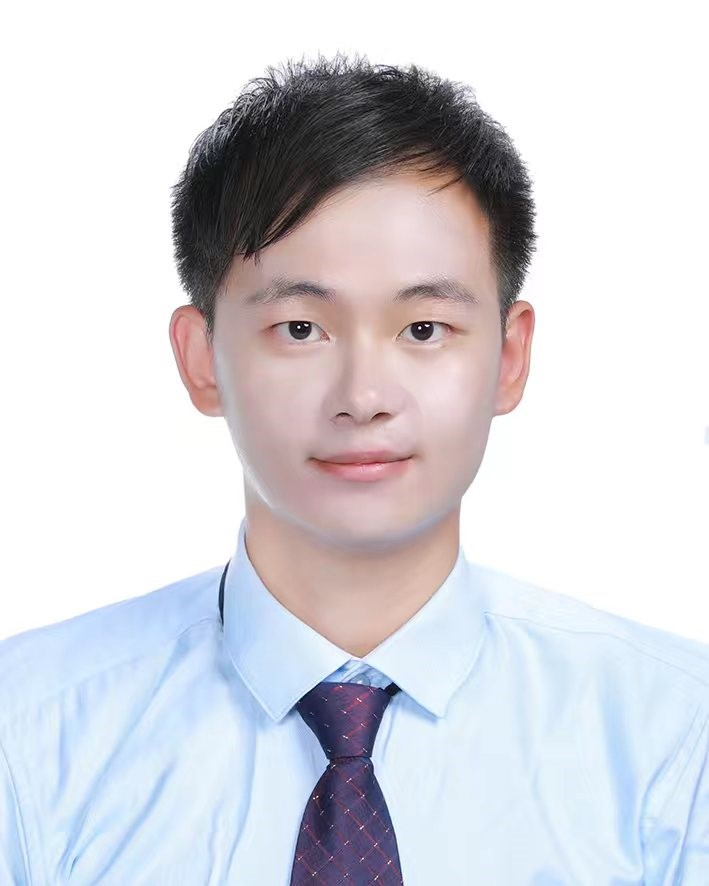
\includegraphics[width=\linewidth]{pic.png}  % 照片路径
    \end{minipage}
    \begin{minipage}{0.65\linewidth}
        \setlength{\tabcolsep}{70pt}
        \def\arraystretch{1.15}
        \begin{tabular}{ll}
            \textbf{\Large{张文杰}}  &  {17704240848} \\
            \textbf{香港科技大学} & \textbf{生命科学 \& 化学} \\
            中共党员 &  \\
        \end{tabular}
    \end{minipage}\hfill
\end{table}

\noindent \colorbox{LightBlue3}{\begin{minipage}{0.99\textwidth}{\textbf{联系方式 \vphantom{p\^{E}}}}\end{minipage}}\\[-0.3cm]
\begin{itemize}[noitemsep,nolistsep]
    \item 邮箱: 17704240848@163.com
    \item 微信: 17704240848
    \item 电话: 17704240848
    \item GitHub: jayzyzy
\end{itemize}

% 第四份：最浅的浅蓝色
\newpage
\begin{table}
    \begin{minipage}{0.15\linewidth}
        % 插入照片
        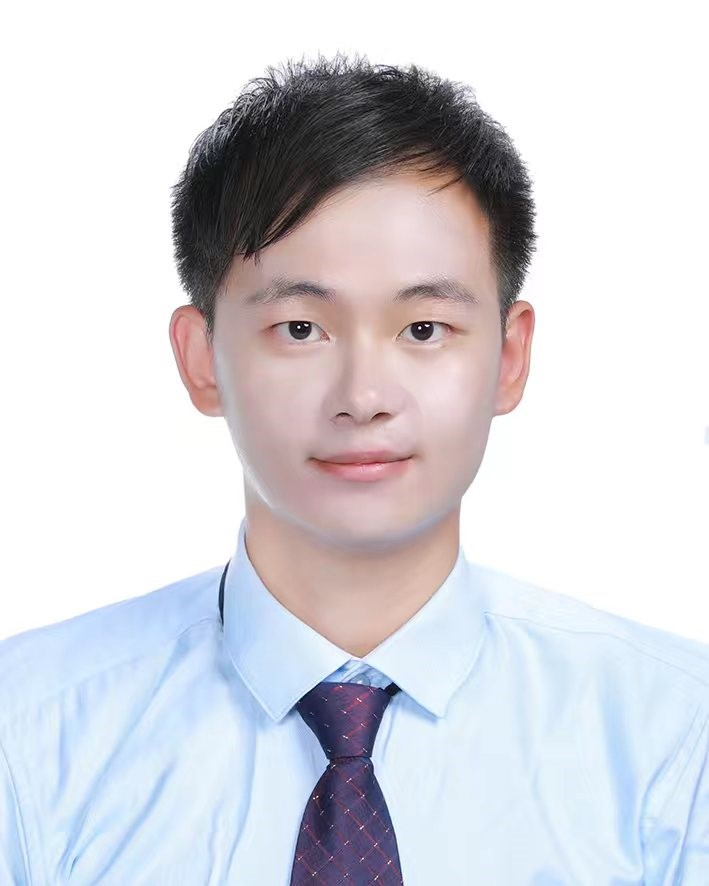
\includegraphics[width=\linewidth]{pic.png}  % 照片路径
    \end{minipage}
    \begin{minipage}{0.65\linewidth}
        \setlength{\tabcolsep}{70pt}
        \def\arraystretch{1.15}
        \begin{tabular}{ll}
            \textbf{\Large{张文杰}}  &  {17704240848} \\
            \textbf{香港科技大学} & \textbf{生命科学 \& 化学} \\
            中共党员 &  \\
        \end{tabular}
    \end{minipage}\hfill
\end{table}

\noindent \colorbox{LightBlue4}{\begin{minipage}{0.99\textwidth}{\textbf{联系方式 \vphantom{p\^{E}}}}\end{minipage}}\\[-0.3cm]
\begin{itemize}[noitemsep,nolistsep]
    \item 邮箱: 17704240848@163.com
    \item 微信: 17704240848
    \item 电话: 17704240848
    \item GitHub: jayzyzy
\end{itemize}

\end{document}